\section{实验目的}
了解数据库应用开发环境的建立与使用;掌握 SQL 语言的使用;通过实践理
解关系数据模型的相关概念;掌握数据库应用开发环境的使用;掌握创建、删除
数据库的方法;掌握创建基本表、查看表属性、修改属性的方法;掌握向表中添
加、删除以及修改数据的方法;掌握查询分析器的使用方法;掌握查询语句在单
表查询中的应用;掌握复杂查询、多表查询的方法;掌握视图的使用方法;巩固
数据库的基础知识.

\section{实验预备内容}
\begin{enumerate}
  \item 阅读教材《数据库系统概论》第三章关系数据库标准语言 SQL.
  \item 阅读实验使用的数据库管理系统的相关参考资料.
\end{enumerate}

\section{实验环境}
\begin{itemize}
  \item OS: Linux
  \item DBMS: OpenGauss DataBase
\end{itemize}

\section{实验内容}

\subsection{所设计的数据库和表的情况简介}

\subsubsection{应用场景}

商家用来管理产品、顾客、订单、供应商等的数据库(commerce).
\begin{enumerate}
  \item 产品数据;
  \item 顾客数据;
  \item 订单数据;
  \item 供应商数据.
\end{enumerate}

\subsubsection{vendors表}
vendors表存储销售产品的供应商.每个供应商在这个表中有一个记录,供应商ID(vend\_id)列用来匹配产品和供应商.
这个表用vend\_id作为主键.vend\_id为自动增量字段.

\begin{table}[H]
  \caption{vendors}
  \begin{center}
    \begin{tabular}[c]{|l|l|}
      \hline
      列 & 说明 \\
      \hline
      vend\_id & 唯一的供应商 ID \\
      \hline
      vend\_name & 供应商名 \\
      \hline
      vend\_address & 供应商的地址 \\
      \hline
      vend\_city & 供应商的城市 \\
      \hline
      vend\_state & 供应商的州 \\
      \hline
      vend\_zip & 供应商的邮政编码 \\
      \hline
      vend\_country & 供应商的国家 \\
      \hline
    \end{tabular}
  \end{center}
\end{table}

\subsubsection{products表}
products表包含产品列表,每行一个产品.每个产品有唯一的ID
(prod\_id列),通过vend\_id(供应商的唯一ID)关联到它的供应商.
这个表用prod\_id作为其主键.同时在vend\_id上定义一个外键,关联到vendors的vend\_id.

\begin{table}[H]
  \caption{products}
  \begin{center}
    \begin{tabular}[c]{|l|l|}
      \hline
      列 & 说明 \\
      \hline
      prod\_id & 唯一的产品ID \\
      \hline
      vend\_id & 产品供应商ID(关联到vendors表中的vend\_id) \\
      \hline
      prod\_name & 产品名 \\
      \hline
      prod\_price & 产品价格 \\
      \hline
      prod\_desc & 产品描述 \\
      \hline
    \end{tabular}
  \end{center}
\end{table}

\subsubsection{customers表}
customers表存储所有顾客信息.每个顾客有唯一ID(cust\_id).这个表用cust\_id作为主键.cust\_id是自动增量字段.

\begin{table}[H]
  \caption{customers}
  \begin{center}
    \begin{tabular}[c]{|l|l|}
      \hline
      列 & 说明 \\
      \hline
      cust\_id & 唯一的顾客ID \\
      \hline
      cust\_name & 顾客名 \\
      \hline
      cust\_address & 顾客的地址 \\
      \hline
      cust\_city & 顾客的城市 \\
      \hline
      cust\_state & 顾客的州 \\
      \hline
      cust\_zip & 顾客的邮政编码 \\
      \hline
      cust\_country & 顾客的国家 \\
      \hline
      cust\_contact & 顾客的联系名 \\
      \hline
      cust\_email & 顾客的联系email地址 \\
      \hline
    \end{tabular}
  \end{center}
\end{table}

\subsubsection{orders表}
orders表存储顾客订单.每个订单编号唯一(order\_num).
订单用cust\_id列(关联到customer表的顾客唯一ID)与相应顾客关联.
这个表用order\_num作为主键.order\_num是自动增量字段.
同时在cust\_id上定义一个外键,关联到customers的cust\_id.

\begin{table}[H]
  \caption{orders}
  \begin{center}
    \begin{tabular}[c]{|l|l|}
      \hline
      列 & 说明 \\
      \hline
      order\_num & 唯一订单号 \\
      \hline
      order\_date & 订单日期 \\
      \hline
      cust\_id & 订单顾客 ID (关系到 customers 表 的cust\_id) \\
      \hline
    \end{tabular}
  \end{center}
\end{table}

\subsubsection{orderitems表}
orderitems表存储每个订单中的实际物品,每个订单的每个物品占
一行.对orders中的每一行,orderitems中有一行或多行.每个订单物
品由订单号加订单物品(第一个物品、第二个物品等)唯一标识.订单
物品通过order\_num列(关联到orders中订单的唯一ID)与它们相应的订
单相关联.

\begin{table}[H]
  \caption{orderitems}
  \begin{center}
    \begin{tabular}[c]{|l|l|}
      \hline
      列 & 说明 \\
      \hline
      order\_num & 订单号(关联到orders表的order\_num) \\
      \hline
      order\_item & 订单物品号(在某个订单中的顺序) \\
      \hline
      prod\_id & 产品ID(关联到products表的prod\_id) \\
      \hline
      quantity & 物品数量 \\
      \hline
      item\_price & 物品价格 \\
      \hline
    \end{tabular}
  \end{center}
\end{table}

\subsubsection{productnotes表}
productnotes表存储与特定产品有关的注释.并非所有产品都有相关的注释,而有的产品可能有许多相关的注释.
这个表用note\_id作为其主键.

\begin{table}[H]
  \caption{productnotes}
  \begin{center}
    \begin{tabular}[c]{|l|l|}
      \hline
      列 & 说明 \\
      \hline
      note\_id & 唯一注释ID \\
      \hline
      prod\_id & 产品ID(对应于products表中的prod\_id) \\
      \hline
      note\_date & 增加注释的日期 \\
      \hline
      note\_text & 注释文本 \\
      \hline
    \end{tabular}
  \end{center}
\end{table}

\subsection{熟悉DBMS实验环境}
了解华为 openGauss 数据库的安装过程及相关工具的使用方法.

\begin{figure}[H]
  \begin{center}
    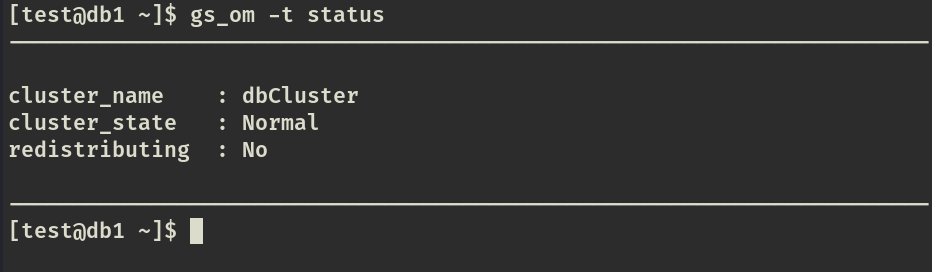
\includegraphics[width=0.95\textwidth,scale=0.5]{./figures/gauss_usage.png}
  \end{center}
  \caption{openGauss 数据库相关工具的使用和安装情况}
\end{figure}

\subsection{创建数据库, 创建并维护基本表的结构和数据}

以下内容使用 SQL 语句完成:

\begin{enumerate}
  \item 设计一个应用场景,创建符合该应用需求的应用数据库.
\begin{center}
\begin{minted}[xleftmargin=5mm]{sql}
-- 应用需求如4.1节所述
create database commerce;
\end{minted}
\end{center}
\begin{figure}[H]
  \begin{center}
    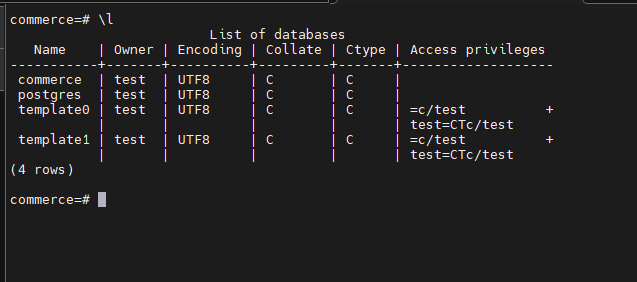
\includegraphics[width=0.95\textwidth,scale=0.5]{./figures/create_database.png}
  \end{center}
  \caption{创建数据库 commerce}
\end{figure}
  \item 在该数据库中创建至少 4 个相互关联的基本表,并设置主键、外键、自定义完整性约束(非空、唯一、默认值、check).
\begin{center}
\begin{minted}[xleftmargin=5mm,breaklines,breakanywhere]{sql}
-- Create customers table
CREATE SEQUENCE customers_id_seq
START WITH 1
INCREMENT BY 1
NO MINVALUE
NO MAXVALUE
CACHE 1;
CREATE TABLE customers
(
  cust_id      int       PRIMARY KEY default nextval('customers_id_seq'::regclass),
  cust_name    char(50)  NOT NULL ,
  cust_address char(50)  NULL ,
  cust_city    char(50)  NULL ,
  cust_state   char(5)   NULL ,
  cust_zip     char(10)  NULL ,
  cust_country char(50)  NULL ,
  cust_contact char(50)  NULL ,
  cust_email   char(255) NULL
);

-- Create orderitems table
CREATE TABLE orderitems
(
  order_num  int          NOT NULL ,
  order_item int          NOT NULL ,
  prod_id    char(10)     NOT NULL ,
  quantity   int          NOT NULL ,
  item_price decimal(8,2) NOT NULL ,
  PRIMARY KEY (order_num, order_item)
);

-- Create orders table
CREATE SEQUENCE orders_id_seq
START WITH 1
INCREMENT BY 1
NO MINVALUE
NO MAXVALUE
CACHE 1;
CREATE TABLE orders
(
  order_num  int      NOT NULL PRIMARY KEY default nextval('orders_id_seq'::regclass),
  order_date date NOT NULL ,
  cust_id    int      NOT NULL
);

-- Create products table
CREATE TABLE products
(
  prod_id    char(10)      NOT NULL,
  vend_id    int           NOT NULL ,
  prod_name  char(255)     NOT NULL ,
  prod_price decimal(8,2)  NOT NULL ,
  prod_desc  text          NULL ,
  PRIMARY KEY(prod_id)
);

-- Create vendors table
CREATE SEQUENCE vendors_id_seq
START WITH 1
INCREMENT BY 1
NO MINVALUE
NO MAXVALUE
CACHE 1;
CREATE TABLE vendors
(
  vend_id      int      NOT NULL PRIMARY KEY default nextval('vendors_id_seq'::regclass),
  vend_name    char(50) NOT NULL ,
  vend_address char(50) NULL ,
  vend_city    char(50) NULL ,
  vend_state   char(5)  NULL ,
  vend_zip     char(10) NULL ,
  vend_country char(50) NULL
);

-- Create productnotes table
CREATE SEQUENCE productnotes_id_seq
START WITH 1
INCREMENT BY 1
NO MINVALUE
NO MAXVALUE
CACHE 1;
CREATE TABLE productnotes
(
  note_id    int           NOT NULL PRIMARY KEY default nextval('productnotes_id_seq'::regclass),
  prod_id    char(10)      NOT NULL,
  note_date date       NOT NULL,
  note_text  text          NULL
);
\end{minted}
\end{center}
\begin{figure}[H]
  \begin{center}
    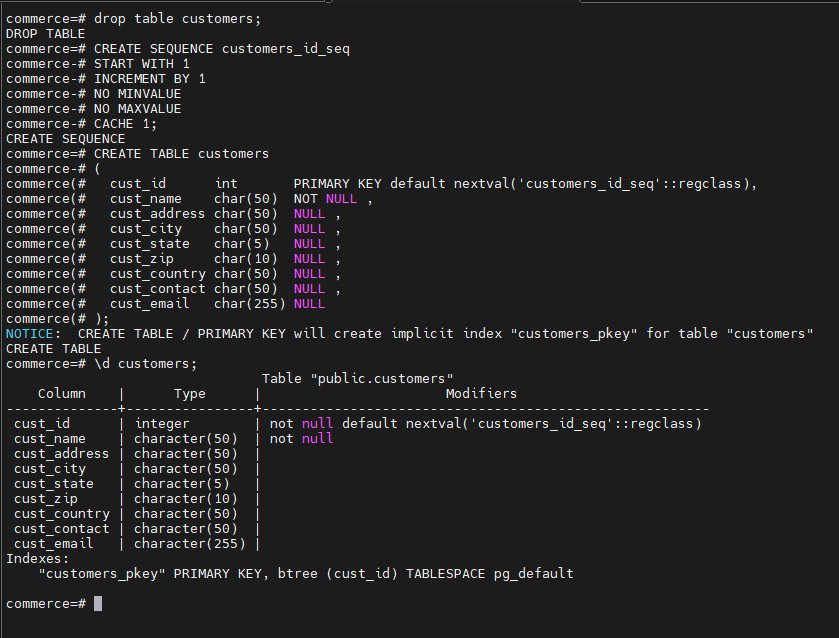
\includegraphics[width=0.95\textwidth,scale=0.5]{./figures/create_table_customers.png}
  \end{center}
  \caption{创建 customers 表}
\end{figure}
\begin{figure}[H]
  \begin{center}
    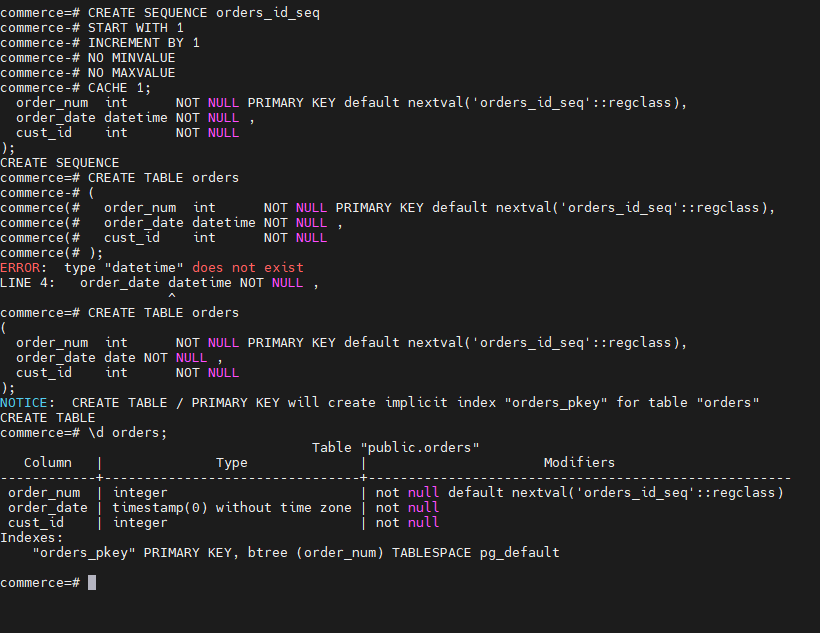
\includegraphics[width=0.95\textwidth,scale=0.5]{./figures/create_table_orders.png}
  \end{center}
  \caption{创建 orders 表}
\end{figure}
\begin{figure}[H]
  \begin{center}
    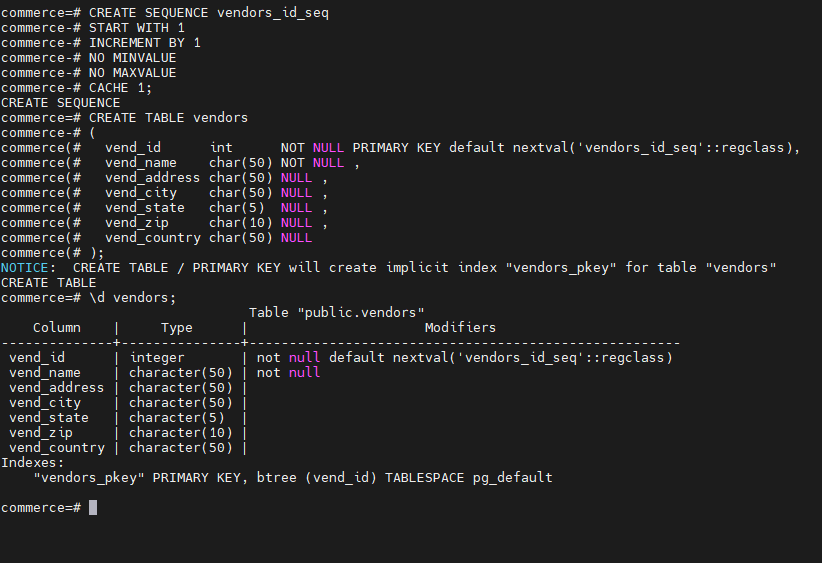
\includegraphics[width=0.95\textwidth,scale=0.5]{./figures/create_table_vendors.png}
  \end{center}
  \caption{创建 vendors 表}
\end{figure}
\begin{figure}[H]
  \begin{center}
    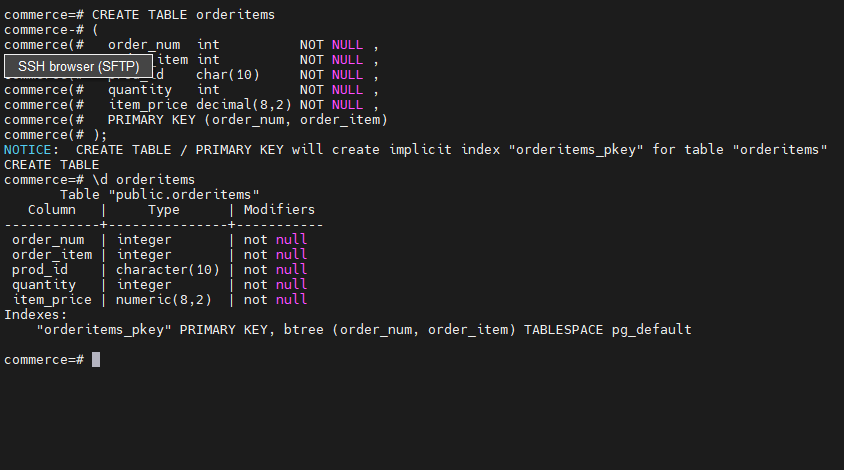
\includegraphics[width=0.95\textwidth,scale=0.5]{./figures/create_table_orderitems.png}
  \end{center}
  \caption{创建 orderitems 表}
\end{figure}
\begin{figure}[H]
  \begin{center}
    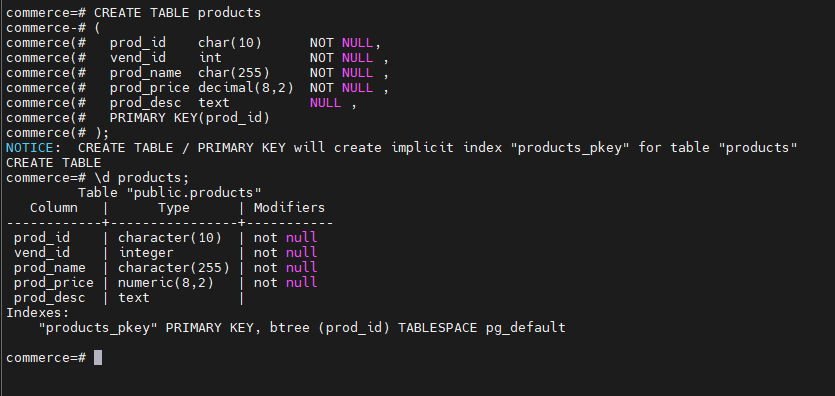
\includegraphics[width=0.95\textwidth,scale=0.5]{./figures/create_table_products.png}
  \end{center}
  \caption{创建 products 表}
\end{figure}
\begin{figure}[H]
  \begin{center}
    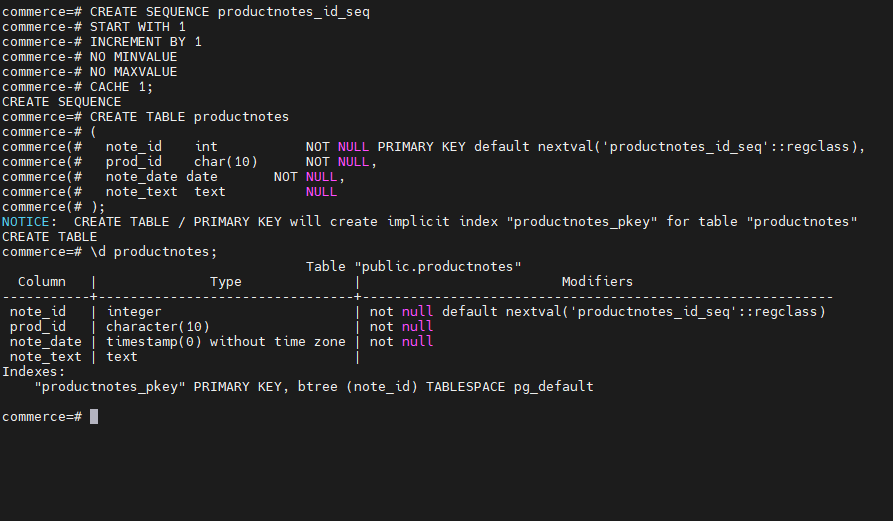
\includegraphics[width=0.95\textwidth,scale=0.5]{./figures/create_table_productnotes.png}
  \end{center}
  \caption{创建 productnotes 表}
\end{figure}
  \item 对表的结构进行修改操作.
\begin{center}
\begin{minted}[xleftmargin=5mm,breaklines,breakanywhere]{sql}
ALTER TABLE orderitems ADD CONSTRAINT fk_orderitems_orders
  FOREIGN KEY (order_num) REFERENCES orders (order_num);
ALTER TABLE orderitems ADD CONSTRAINT fk_orderitems_products
  FOREIGN KEY (prod_id) REFERENCES products (prod_id);
ALTER TABLE orders ADD CONSTRAINT fk_orders_customers
  FOREIGN KEY (cust_id) REFERENCES customers (cust_id);
ALTER TABLE products ADD CONSTRAINT fk_products_vendors
  FOREIGN KEY (vend_id) REFERENCES vendors (vend_id);
\end{minted}
\end{center}
\begin{figure}[H]
  \begin{center}
    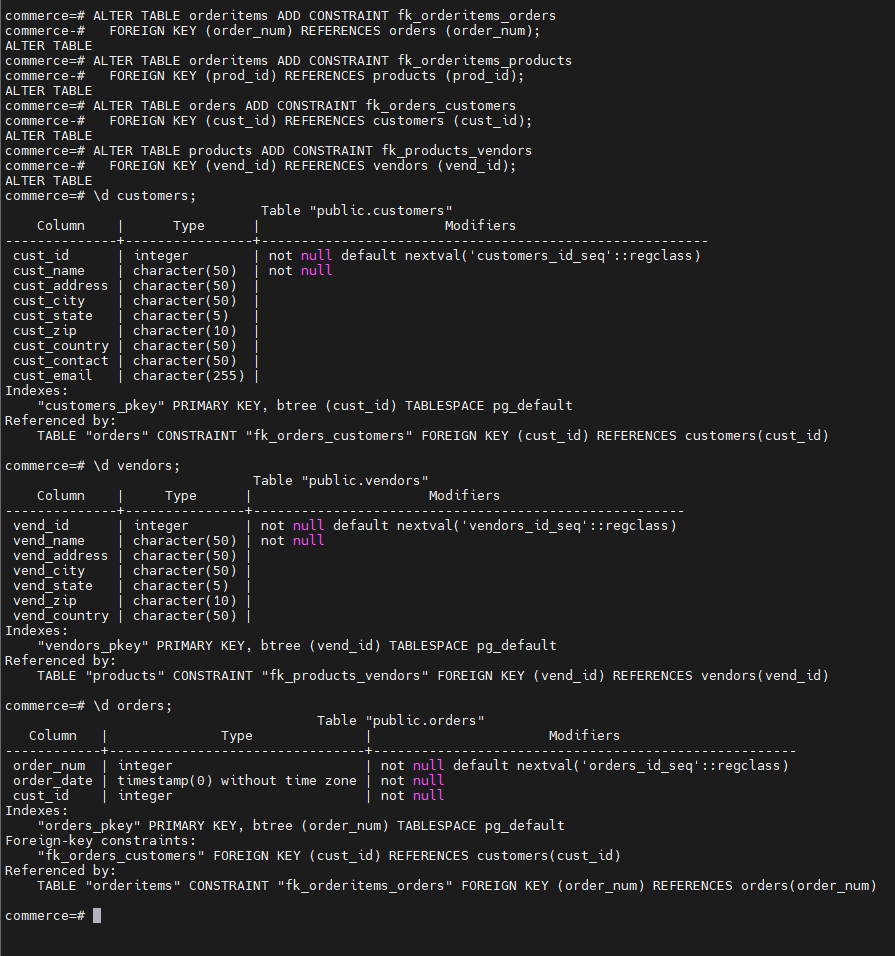
\includegraphics[width=0.95\textwidth,scale=0.5]{./figures/alter_table.png}
  \end{center}
  \caption{对表进行修改操作}
\end{figure}
  \item 创建索引及删除索引.
\begin{center}
\begin{minted}[xleftmargin=5mm,breaklines,breakanywhere]{sql}
CREATE INDEX product_index ON products(prod_name);
DROP INDEX product_index;
\end{minted}
\end{center}
\begin{figure}[H]
  \begin{center}
    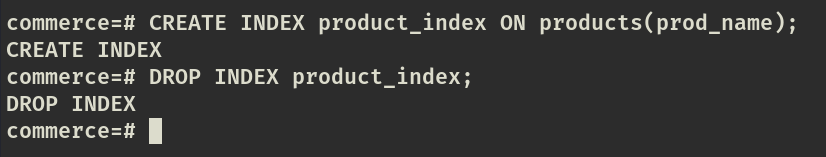
\includegraphics[width=0.95\textwidth,scale=0.5]{./figures/create_and_drop_index.png}
  \end{center}
  \caption{创建及删除索引}
\end{figure}
  \item 向表中录入若干数据,对表中数据进行修改和删除操作.
\begin{center}
\begin{minted}[xleftmargin=5mm,breaklines,breakanywhere]{sql}
-- Customers table
INSERT INTO customers(cust_id, cust_name, cust_address, cust_city, cust_state, cust_zip, cust_country, cust_contact, cust_email)
VALUES(10001, 'Coyote Inc.', '200 Maple Lane', 'Detroit', 'MI', '44444', 'USA', 'Y Lee', 'ylee@coyote.com');
INSERT INTO customers(cust_id, cust_name, cust_address, cust_city, cust_state, cust_zip, cust_country, cust_contact)
VALUES(10002, 'Mouse House', '333 Fromage Lane', 'Columbus', 'OH', '43333', 'USA', 'Jerry Mouse');
INSERT INTO customers(cust_id, cust_name, cust_address, cust_city, cust_state, cust_zip, cust_country, cust_contact, cust_email)
VALUES(10003, 'Wascals', '1 Sunny Place', 'Muncie', 'IN', '42222', 'USA', 'Jim Jones', 'rabbit@wascally.com');
INSERT INTO customers(cust_id, cust_name, cust_address, cust_city, cust_state, cust_zip, cust_country, cust_contact, cust_email)
VALUES(10004, 'Yosemite Place', '829 Riverside Drive', 'Phoenix', 'AZ', '88888', 'USA', 'Y Sam', 'sam@yosemite.com');
INSERT INTO customers(cust_id, cust_name, cust_address, cust_city, cust_state, cust_zip, cust_country, cust_contact)
VALUES(10005, 'E Fudd', '4545 53rd Street', 'Chicago', 'IL', '54545', 'USA', 'E Fudd');

-- Vendors table
INSERT INTO vendors(vend_id, vend_name, vend_address, vend_city, vend_state, vend_zip, vend_country)
VALUES(1001,'Anvils R Us','123 Main Street','Southfield','MI','48075', 'USA');
INSERT INTO vendors(vend_id, vend_name, vend_address, vend_city, vend_state, vend_zip, vend_country)
VALUES(1002,'LT Supplies','500 Park Street','Anytown','OH','44333', 'USA');
INSERT INTO vendors(vend_id, vend_name, vend_address, vend_city, vend_state, vend_zip, vend_country)
VALUES(1003,'ACME','555 High Street','Los Angeles','CA','90046', 'USA');
INSERT INTO vendors(vend_id, vend_name, vend_address, vend_city, vend_state, vend_zip, vend_country)
VALUES(1004,'Furball Inc.','1000 5th Avenue','New York','NY','11111', 'USA');
INSERT INTO vendors(vend_id, vend_name, vend_address, vend_city, vend_state, vend_zip, vend_country)
VALUES(1005,'Jet Set','42 Galaxy Road','London', NULL,'N16 6PS', 'England');
INSERT INTO vendors(vend_id, vend_name, vend_address, vend_city, vend_state, vend_zip, vend_country)
VALUES(1006,'Jouets Et Ours','1 Rue Amusement','Paris', NULL,'45678', 'France');

-- Products table
INSERT INTO products(prod_id, vend_id, prod_name, prod_price, prod_desc)
VALUES('ANV01', 1001, '.5 ton anvil', 5.99, '.5 ton anvil, black, complete with handy hook');
INSERT INTO products(prod_id, vend_id, prod_name, prod_price, prod_desc)
VALUES('ANV02', 1001, '1 ton anvil', 9.99, '1 ton anvil, black, complete with handy hook and carrying case');
INSERT INTO products(prod_id, vend_id, prod_name, prod_price, prod_desc)
VALUES('ANV03', 1001, '2 ton anvil', 14.99, '2 ton anvil, black, complete with handy hook and carrying case');
INSERT INTO products(prod_id, vend_id, prod_name, prod_price, prod_desc)
VALUES('OL1', 1002, 'Oil can', 8.99, 'Oil can, red');
INSERT INTO products(prod_id, vend_id, prod_name, prod_price, prod_desc)
VALUES('FU1', 1002, 'Fuses', 3.42, '1 dozen, extra long');
INSERT INTO products(prod_id, vend_id, prod_name, prod_price, prod_desc)
VALUES('SLING', 1003, 'Sling', 4.49, 'Sling, one size fits all');
INSERT INTO products(prod_id, vend_id, prod_name, prod_price, prod_desc)
VALUES('TNT1', 1003, 'TNT (1 stick)', 2.50, 'TNT, red, single stick');
INSERT INTO products(prod_id, vend_id, prod_name, prod_price, prod_desc)
VALUES('TNT2', 1003, 'TNT (5 sticks)', 10, 'TNT, red, pack of 10 sticks');
INSERT INTO products(prod_id, vend_id, prod_name, prod_price, prod_desc)
VALUES('FB', 1003, 'Bird seed', 10, 'Large bag (suitable for road runners)');
INSERT INTO products(prod_id, vend_id, prod_name, prod_price, prod_desc)
VALUES('FC', 1003, 'Carrots', 2.50, 'Carrots (rabbit hunting season only)');
INSERT INTO products(prod_id, vend_id, prod_name, prod_price, prod_desc)
VALUES('SAFE', 1003, 'Safe', 50, 'Safe with combination lock');
INSERT INTO products(prod_id, vend_id, prod_name, prod_price, prod_desc)
VALUES('DTNTR', 1003, 'Detonator', 13, 'Detonator (plunger powered), fuses not included');
INSERT INTO products(prod_id, vend_id, prod_name, prod_price, prod_desc)
VALUES('JP1000', 1005, 'JetPack 1000', 35, 'JetPack 1000, intended for single use');
INSERT INTO products(prod_id, vend_id, prod_name, prod_price, prod_desc)
VALUES('JP2000', 1005, 'JetPack 2000', 55, 'JetPack 2000, multi-use');

-- Orders table
INSERT INTO orders(order_num, order_date, cust_id)
VALUES(20005, '2005-09-01', 10001);
INSERT INTO orders(order_num, order_date, cust_id)
VALUES(20006, '2005-09-12', 10003);
INSERT INTO orders(order_num, order_date, cust_id)
VALUES(20007, '2005-09-30', 10004);
INSERT INTO orders(order_num, order_date, cust_id)
VALUES(20008, '2005-10-03', 10005);
INSERT INTO orders(order_num, order_date, cust_id)
VALUES(20009, '2005-10-08', 10001);

-- Orderitems table
INSERT INTO orderitems(order_num, order_item, prod_id, quantity, item_price)
VALUES(20005, 1, 'ANV01', 10, 5.99);
INSERT INTO orderitems(order_num, order_item, prod_id, quantity, item_price)
VALUES(20005, 2, 'ANV02', 3, 9.99);
INSERT INTO orderitems(order_num, order_item, prod_id, quantity, item_price)
VALUES(20005, 3, 'TNT2', 5, 10);
INSERT INTO orderitems(order_num, order_item, prod_id, quantity, item_price)
VALUES(20005, 4, 'FB', 1, 10);
INSERT INTO orderitems(order_num, order_item, prod_id, quantity, item_price)
VALUES(20006, 1, 'JP2000', 1, 55);
INSERT INTO orderitems(order_num, order_item, prod_id, quantity, item_price)
VALUES(20007, 1, 'TNT2', 100, 10);
INSERT INTO orderitems(order_num, order_item, prod_id, quantity, item_price)
VALUES(20008, 1, 'FC', 50, 2.50);
INSERT INTO orderitems(order_num, order_item, prod_id, quantity, item_price)
VALUES(20009, 1, 'FB', 1, 10);
INSERT INTO orderitems(order_num, order_item, prod_id, quantity, item_price)
VALUES(20009, 2, 'OL1', 1, 8.99);
INSERT INTO orderitems(order_num, order_item, prod_id, quantity, item_price)
VALUES(20009, 3, 'SLING', 1, 4.49);
INSERT INTO orderitems(order_num, order_item, prod_id, quantity, item_price)
VALUES(20009, 4, 'ANV03', 1, 14.99);

-- Productnotes table
INSERT INTO productnotes(note_id, prod_id, note_date, note_text)
VALUES(101, 'TNT2', '2005-08-17',
'Customer complaint:
Sticks not individually wrapped, too easy to mistakenly detonate all at once.
Recommend individual wrapping.'
);
INSERT INTO productnotes(note_id, prod_id, note_date, note_text)
VALUES(102, 'OL1', '2005-08-18',
'Can shipped full, refills not available.
Need to order new can if refill needed.'
);
INSERT INTO productnotes(note_id, prod_id, note_date, note_text)
VALUES(103, 'SAFE', '2005-08-18',
'Safe is combination locked, combination not provided with safe.
This is rarely a problem as safes are typically blown up or dropped by customers.'
);
INSERT INTO productnotes(note_id, prod_id, note_date, note_text)
VALUES(104, 'FC', '2005-08-19',
'Quantity varies, sold by the sack load.
All guaranteed to be bright and orange, and suitable for use as rabbit bait.'
);
INSERT INTO productnotes(note_id, prod_id, note_date, note_text)
VALUES(105, 'TNT2', '2005-08-20',
'Included fuses are short and have been known to detonate too quickly for some customers.
Longer fuses are available (item FU1) and should be recommended.'
);
INSERT INTO productnotes(note_id, prod_id, note_date, note_text)
VALUES(106, 'TNT2', '2005-08-22',
'Matches not included, recommend purchase of matches or detonator (item DTNTR).'
);
INSERT INTO productnotes(note_id, prod_id, note_date, note_text)
VALUES(107, 'SAFE', '2005-08-23',
'Please note that no returns will be accepted if safe opened using explosives.'
);
INSERT INTO productnotes(note_id, prod_id, note_date, note_text)
VALUES(108, 'ANV01', '2005-08-25',
'Multiple customer returns, anvils failing to drop fast enough or falling backwards on purchaser. Recommend that customer considers using heavier anvils.'
);
INSERT INTO productnotes(note_id, prod_id, note_date, note_text)
VALUES(109, 'ANV03', '2005-09-01',
'Item is extremely heavy. Designed for dropping, not recommended for use with slings, ropes, pulleys, or tightropes.'
);
INSERT INTO productnotes(note_id, prod_id, note_date, note_text)
VALUES(110, 'FC', '2005-09-01',
'Customer complaint: rabbit has been able to detect trap, food apparently less effective now.'
);
INSERT INTO productnotes(note_id, prod_id, note_date, note_text)
VALUES(111, 'SLING', '2005-09-02',
'Shipped unassembled, requires common tools (including oversized hammer).'
);
iNSERT INTO productnotes(note_id, prod_id, note_date, note_text)
VALUES(112, 'SAFE', '2005-09-02',
'Customer complaint:
Circular hole in safe floor can apparently be easily cut with handsaw.'
);
INSERT INTO productnotes(note_id, prod_id, note_date, note_text)
VALUES(113, 'ANV01', '2005-09-05',
'Customer complaint:
Not heavy enough to generate flying stars around head of victim. If being purchased for dropping, recommend ANV02 or ANV03 instead.'
);
INSERT INTO productnotes(note_id, prod_id, note_date, note_text)
VALUES(114, 'SAFE', '2005-09-07',
'Call from individual trapped in safe plummeting to the ground, suggests an escape hatch be added.
Comment forwarded to vendor.'
);

-- 更新数据
UPDATE customers
SET cust_name = 'The Fudds',
    cust_email = 'elmer@fudd.com'
WHERE cust_id = 10005;

-- 删除数据
DELETE FROM customers WHERE cust_id = 10006;
\end{minted}
\end{center}
%\begin{figure}[H]
  %\begin{center}
    %\includegraphics[width=0.95\textwidth,scale=0.5]{./figures/}
  %\end{center}
  %\caption{}
%\end{figure}
\begin{figure}[H]
  \begin{center}
    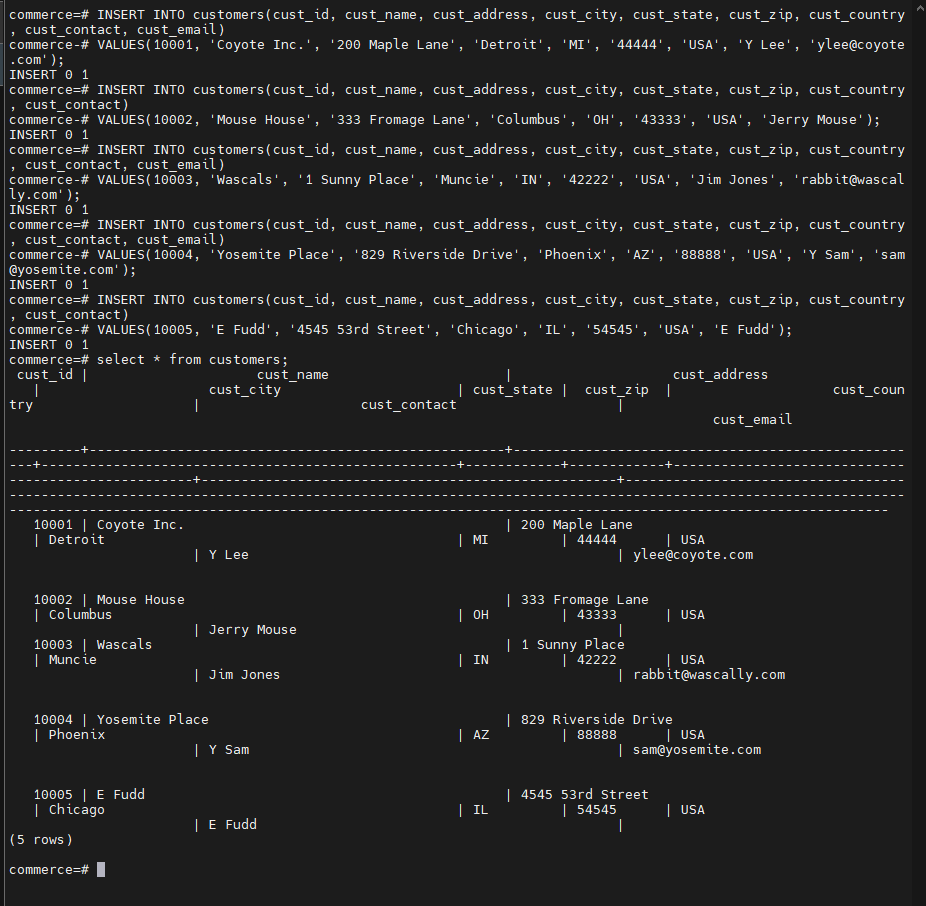
\includegraphics[width=0.95\textwidth,scale=0.5]{./figures/insert_table_customers.png}
  \end{center}
  \caption{向 customers 表插入数据}
\end{figure}
\begin{figure}[H]
  \begin{center}
    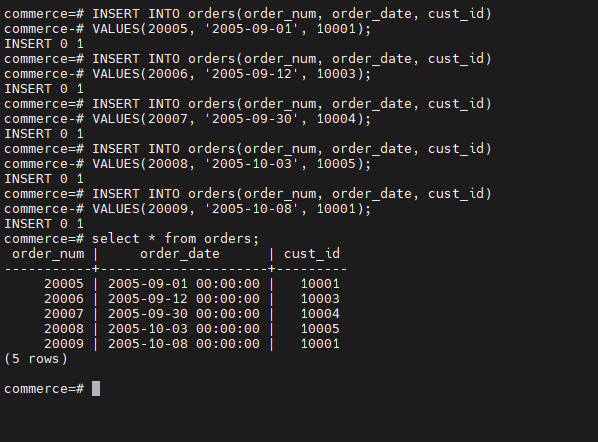
\includegraphics[width=0.95\textwidth,scale=0.5]{./figures/insert_table_orders.png}
  \end{center}
  \caption{向 orders 表插入数据}
\end{figure}
\begin{figure}[H]
  \begin{center}
    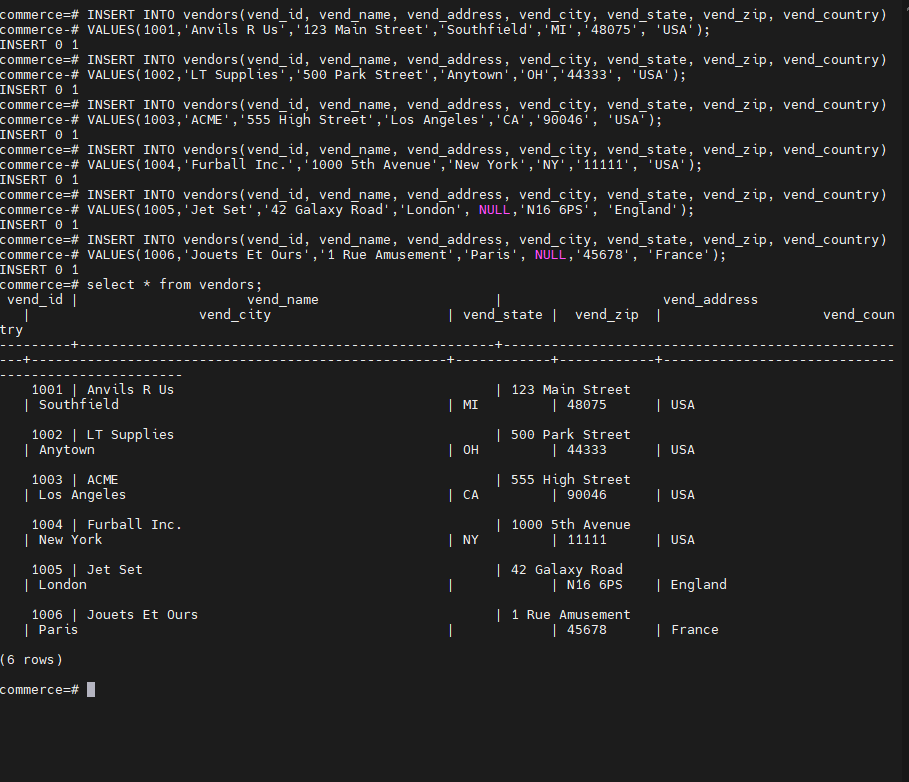
\includegraphics[width=0.95\textwidth,scale=0.5]{./figures/insert_table_vendors.png}
  \end{center}
  \caption{向 vendors 表插入数据}
\end{figure}
\begin{figure}[H]
  \begin{center}
    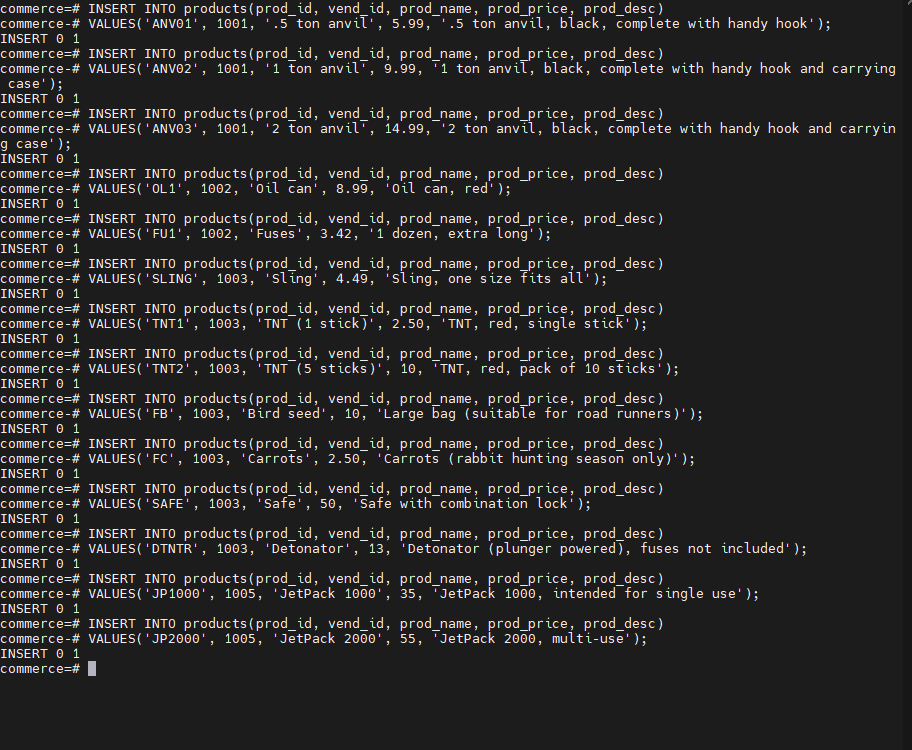
\includegraphics[width=0.95\textwidth,scale=0.5]{./figures/insert_table_products.png}
  \end{center}
  \caption{向 products 表插入数据}
\end{figure}
\begin{figure}[H]
  \begin{center}
    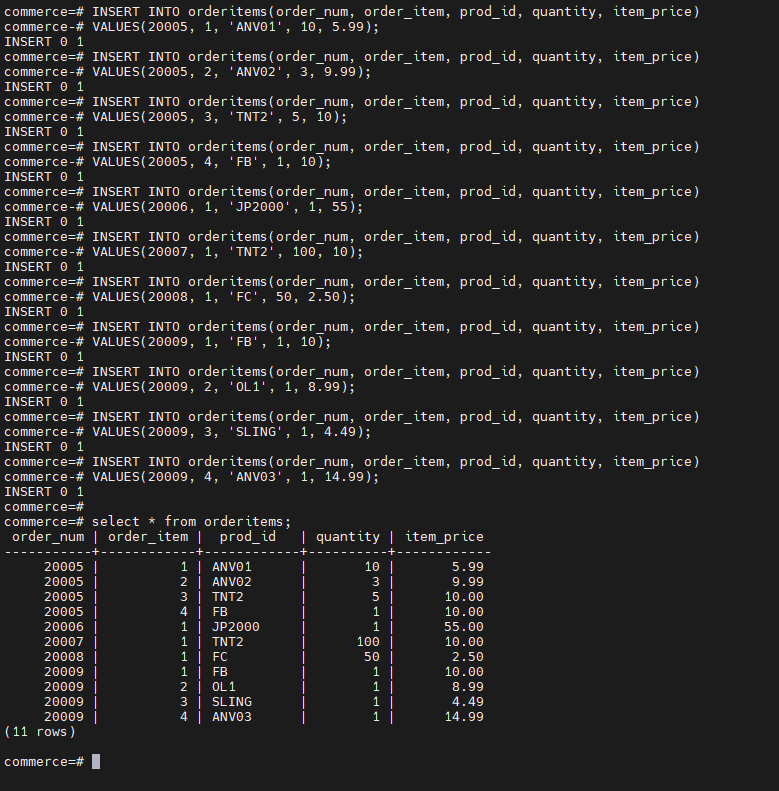
\includegraphics[width=0.95\textwidth,scale=0.5]{./figures/insert_table_orderitems.png}
  \end{center}
  \caption{向 orderitems 表插入数据}
\end{figure}
\begin{figure}[H]
  \begin{center}
    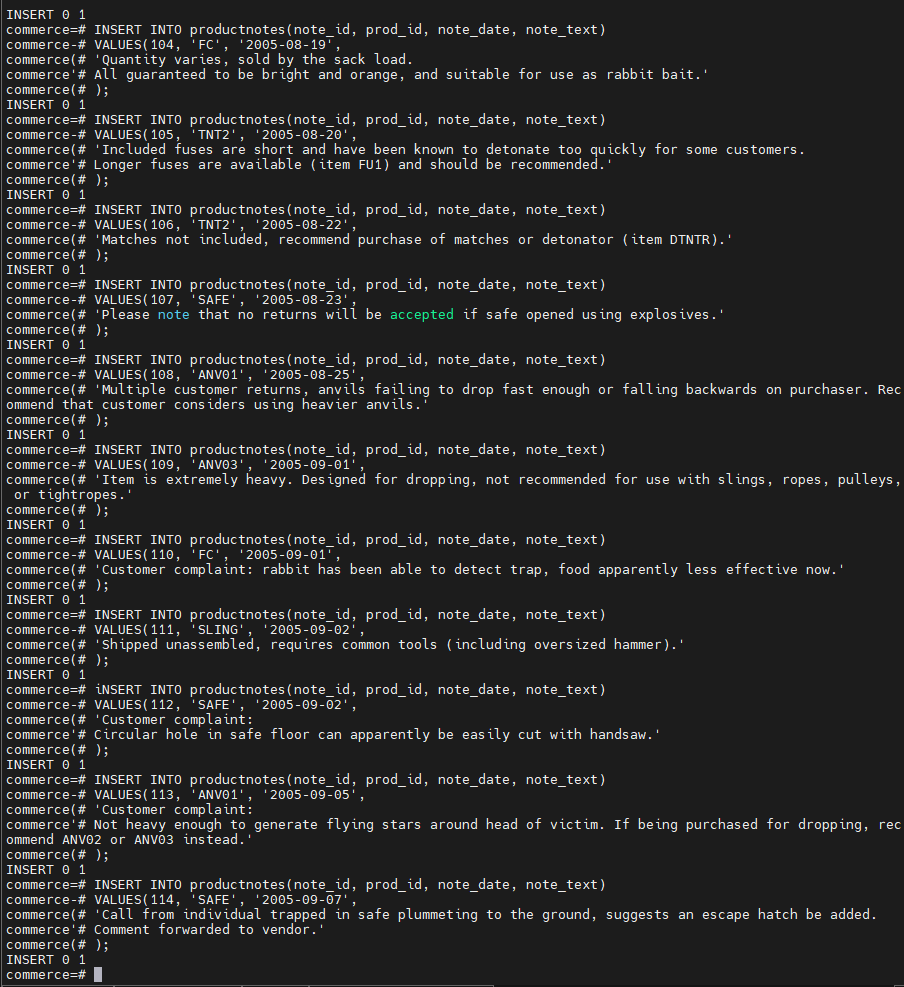
\includegraphics[width=0.95\textwidth,scale=0.5]{./figures/insert_table_productnotes.png}
  \end{center}
  \caption{向 productnotes 表插入数据}
\end{figure}
\begin{figure}[H]
  \begin{center}
    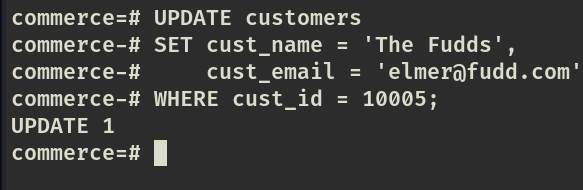
\includegraphics[width=0.95\textwidth,scale=0.5]{./figures/update_customers.png}
  \end{center}
  \caption{更新 customers 表中的数据}
\end{figure}
\begin{figure}[H]
  \begin{center}
    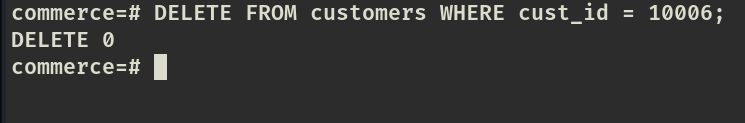
\includegraphics[width=0.95\textwidth,scale=0.5]{./figures/delete_customers.png}
  \end{center}
  \caption{删除 customers 表中的数据}
\end{figure}
\end{enumerate}

\subsection{数据库查询,视图使用}

在创建的表中自行设计实现以下查询:

\begin{enumerate}
  \item 单表查询.
\begin{center}
\begin{minted}[xleftmargin=5mm,breaklines,breakanywhere]{sql}
SELECT prod_id, prod_name, prod_price FROM products;
\end{minted}
\end{center}
\begin{figure}[H]
  \begin{center}
    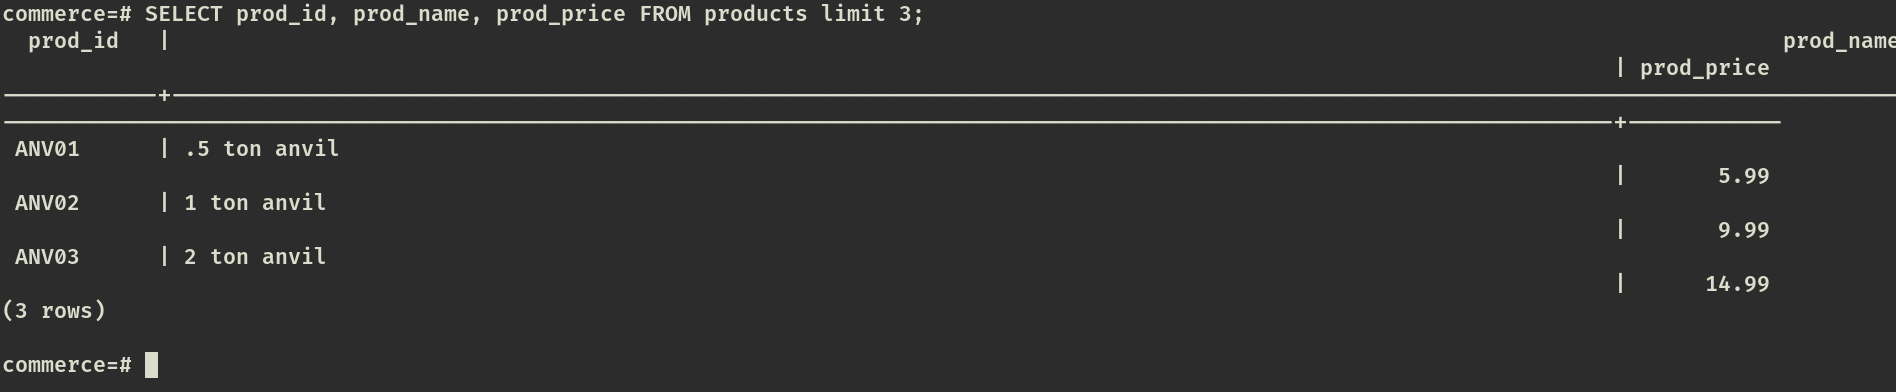
\includegraphics[width=0.95\textwidth,scale=0.5]{./figures/single_select.png}
  \end{center}
  \caption{单表查询}
\end{figure}
  \item 多表连接查询并排序输出.
\begin{center}
\begin{minted}[xleftmargin=5mm,breaklines,breakanywhere]{sql}
SELECT vend_name, prod_name, prod_price
FROM vendors, products
WHERE vendors.vend_id = products.vend_id
ORDER BY vend_name, prod_name;
\end{minted}
\end{center}
\begin{figure}[H]
  \begin{center}
    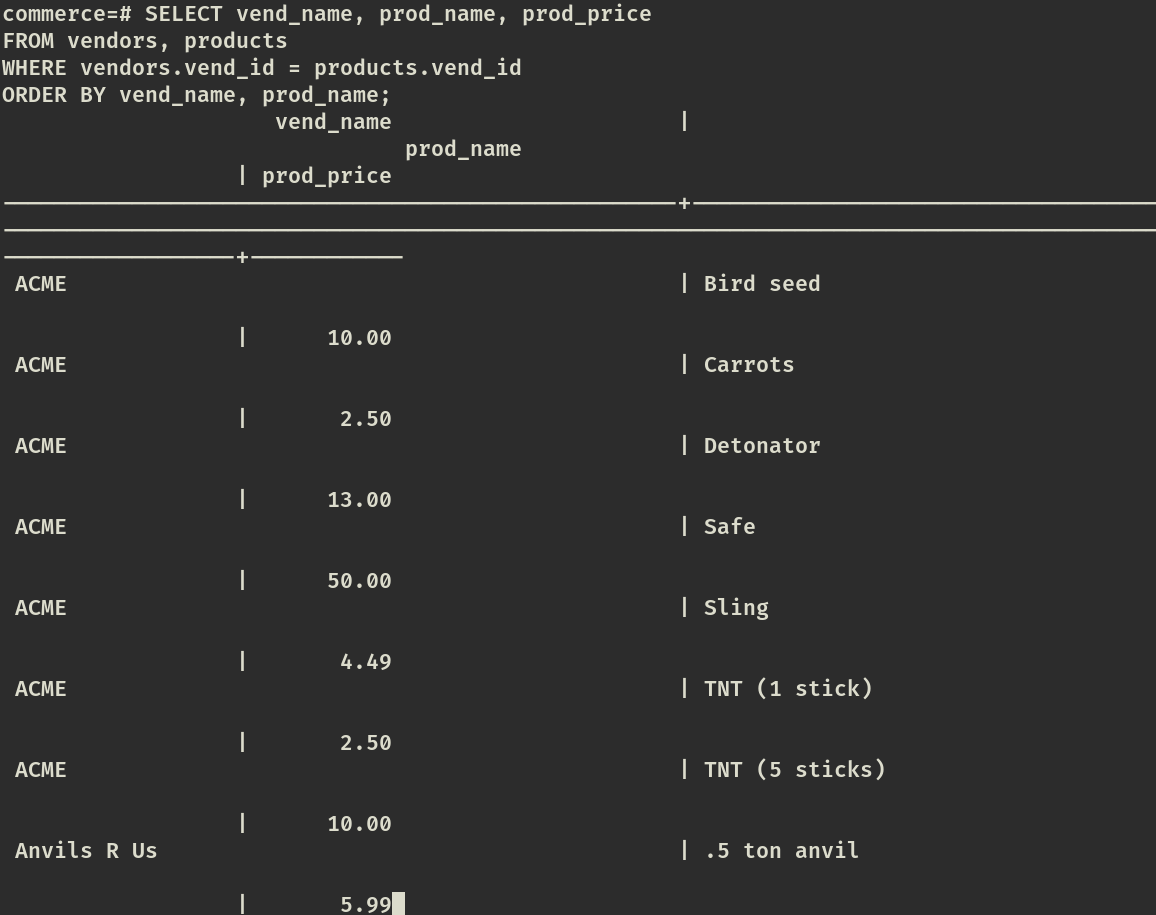
\includegraphics[width=0.95\textwidth,scale=0.5]{./figures/multiple_select.png}
  \end{center}
  \caption{多表连接查询并排序输出}
\end{figure}
  \item 使用聚集函数的查询.
\begin{center}
\begin{minted}[xleftmargin=5mm,breaklines,breakanywhere]{sql}
SELECT COUNT(*) AS num_cust FROM customers;
\end{minted}
\end{center}
\begin{figure}[H]
  \begin{center}
    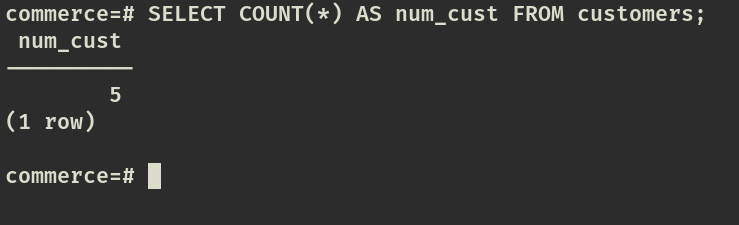
\includegraphics[width=0.95\textwidth,scale=0.5]{./figures/count.png}
  \end{center}
  \caption{使用聚集函数的查询}
\end{figure}
  \item 分组查询.
\begin{center}
\begin{minted}[xleftmargin=5mm,breaklines,breakanywhere]{sql}
SELECT vend_id, COUNT(*) AS num_prods FROM products
GROUP BY vend_id;
\end{minted}
\end{center}
\begin{figure}[H]
  \begin{center}
    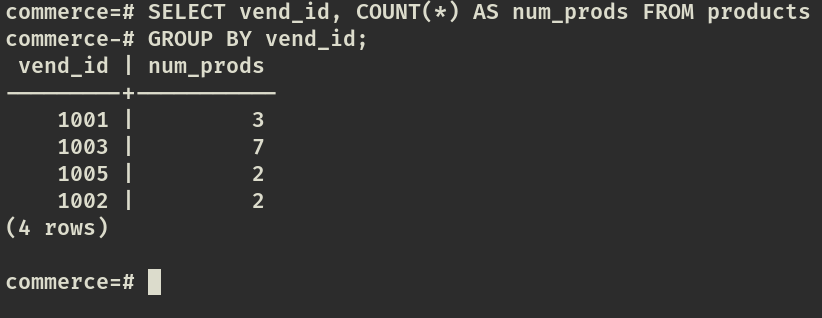
\includegraphics[width=0.95\textwidth,scale=0.5]{./figures/group_by.png}
  \end{center}
  \caption{分组查询}
\end{figure}
  \item 嵌套查询.
\begin{center}
\begin{minted}[xleftmargin=5mm,breaklines,breakanywhere]{sql}
SELECT cust_name, cust_contact FROM customers
WHERE cust_id IN (SELECT cust_id FROM orders
  WHERE order_num IN (SELECT order_num FROM orderitems
    WHERE prod_id = 'TNT2'));
\end{minted}
\end{center}
\begin{figure}[H]
  \begin{center}
    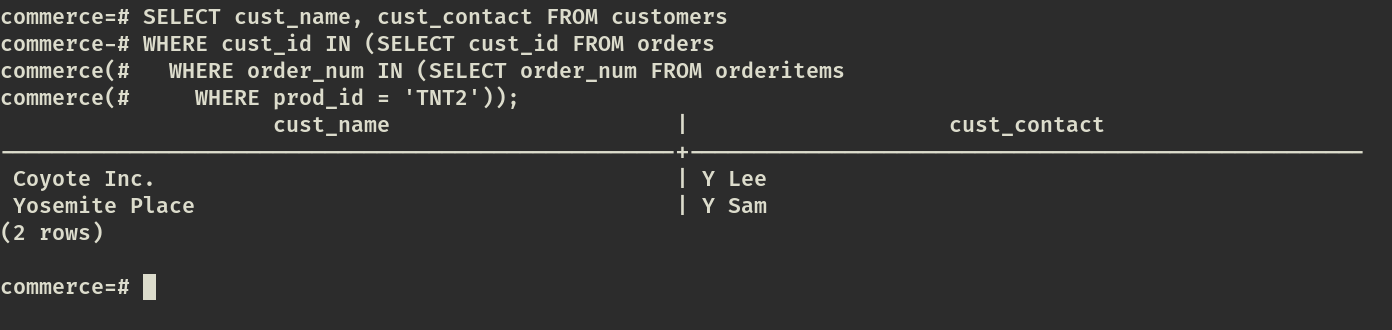
\includegraphics[width=0.95\textwidth,scale=0.5]{./figures/nested_select.png}
  \end{center}
  \caption{嵌套查询}
\end{figure}
  \item 创建并使用视图查询.
\begin{center}
\begin{minted}[xleftmargin=5mm,breaklines,breakanywhere]{sql}
-- 创建视图
CREATE VIEW productcustomers AS
SELECT cust_name, cust_contact, prod_id
FROM customers, orders, orderitems
WHERE customers.cust_id = orders.cust_id
AND orderitems.order_num = orders.order_num;

-- 查询
SELECT cust_name, cust_contact FROM productcustomers WHERE prod_id = 'TNT2';
\end{minted}
\end{center}
\begin{figure}[H]
  \begin{center}
    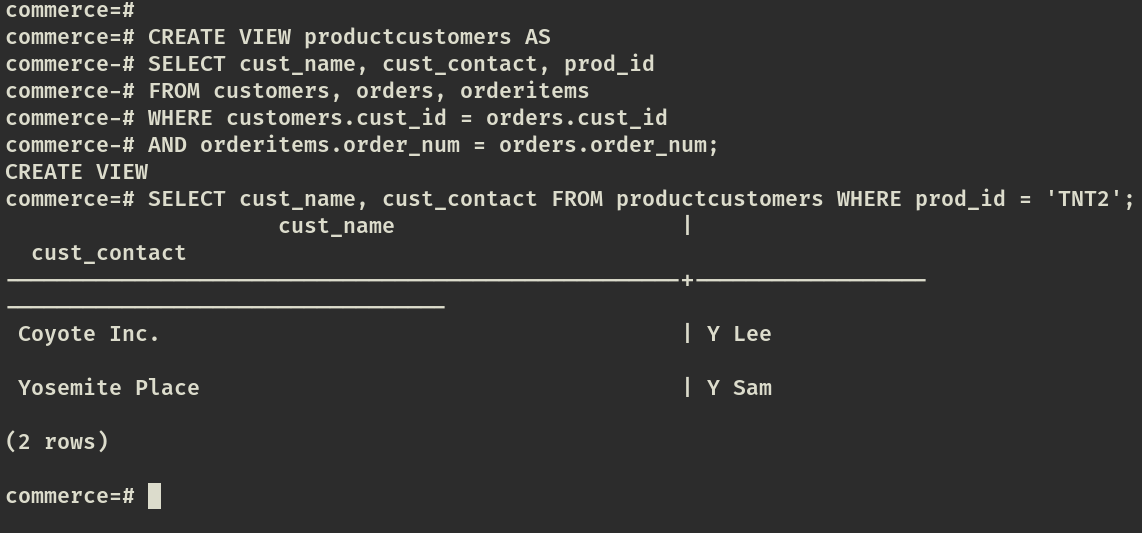
\includegraphics[width=0.95\textwidth,scale=0.5]{./figures/create_view.png}
  \end{center}
  \caption{创建并使用视图查询}
\end{figure}
\end{enumerate}

\subsection{实验总结}

\subsubsection{实验涉及的相关知识}

\begin{itemize}
  \item Linux 命令的使用.
  \item openGauss 数据库的安装和基本使用.
  \item 数据库的创建.
  \item 表的创建和修改.
  \item 索引的创建和删除.
  \item 视图的创建和使用.
  \item 表的完整性及其约束的设计.
  \item 表的数据的插入、更新、删除.
  \item 单表查询.
  \item 多表连接查询.
  \item 嵌套查询.
  \item 聚合查询.
\end{itemize}

\subsubsection{实验遇到的问题及其解决}
没有问题.
